% https://www.sharelatex.com/blog/2013/08/27/tikz-series-pt1.html
\documentclass[beamer]{standalone}
\definecolor{printred}{RGB}{215,25,28}
\definecolor{printblue}{RGB}{43,131,186}
\usepackage{tikz}
\usetikzlibrary{patterns}
\begin{document}
\newcommand{\drawstencil}[2]{%
  \draw[darkgray, thick, pattern=north west lines, pattern color=gray] (#1-1, #2) rectangle (#1+2, #2+1);
  \draw[darkgray, thick, pattern=north west lines, pattern color=gray] (#1, #2-1) rectangle (#1+1, #2+2);
  \draw[darkgray, thick, pattern=north east lines, pattern color=gray](#1, #2) rectangle (#1+1, #2+1);
}
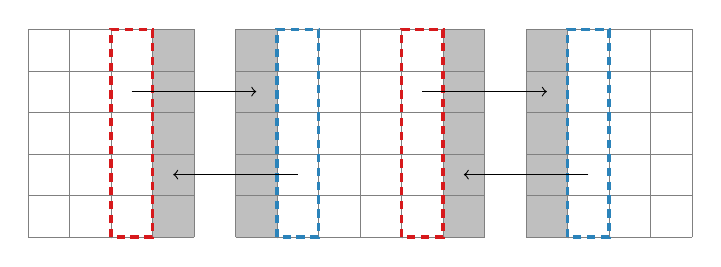
\begin{tikzpicture}[x=1.5em,y=1.5em]

  \fill[lightgray](-2,0) rectangle (-1, 5);
  \fill[lightgray] (0,0) rectangle (1,5);
  \fill[lightgray] (5,0) rectangle (6,5);
  \fill[lightgray](7,0) rectangle (8, 5);

  % Grids
  \draw[step=1, gray, very thin] (-5,0) grid (-1, 5);
  \draw[step=1, gray, very thin] (0,0) grid (6, 5);
  \draw[step=1, gray, very thin] (7,0) grid (11, 5);

  \onslide<1> {
    \drawstencil{1}{2} 
  }
  \onslide<2> {
    % Left-To-Right transmission (->)
    \draw[printred, densely dashed, very thick](-3,0) rectangle (-2, 5);
    \draw[->] (-2.5,3.5) -- (0.5,3.5);
    \draw[printred, densely dashed, very thick](4,0) rectangle (5, 5);
    \draw[->] (4.5,3.5) -- (7.5,3.5);

    % Right-To-Left transmission (<-)
    \draw[printblue, densely dashed, very thick] (1,0) rectangle (2,5);
    \draw[->] (1.5, 1.5) -- (-1.5, 1.5);
    \draw[printblue, densely dashed, very thick] (8,0) rectangle (9,5);
    \draw[->] (8.5, 1.5) -- (5.5, 1.5);
  }

\end{tikzpicture}
\end{document}
